% !TEX TS-program = XeLaTeX

% STYLE

\documentclass[a4paper, 12pt]{article}
\usepackage[left=3cm,
		    right=3cm,
    		    top=3cm,
		    bottom=3cm,
		    bindingoffset=0cm]{geometry}
		    \usepackage{array}
\usepackage{float}
\usepackage{graphicx}
\graphicspath{ {./images/} }
\usepackage{subfig}
\usepackage{enumerate}
\usepackage[normalem]{ulem} % underlining
\usepackage{booktabs} % tables
\usepackage{epigraph}  
\usepackage{multirow}  
\PassOptionsToPackage{table}{xcolor}% coloring tables

% LANGUAGE + FONT
		    
\usepackage[english]{babel}
\usepackage[backend=biber,
                     style=unified]{biblatex}
\newcommand{\citeay}[2][]{
   \citeauthor{#2} (\citeyear[#1]{#2})}
\addbibresource{ref.bib}
\usepackage{fontspec}  
\setmainfont{Minion 3}

% DRAWING

\usepackage{tikz}
\usepackage{tikz-qtree}
\usetikzlibrary{shapes.geometric}
\usetikzlibrary{trees,arrows}
\usetikzlibrary{positioning}
\usetikzlibrary{matrix}
\usetikzlibrary{tikzmark}
\usetikzlibrary{decorations.shapes}
\usetikzlibrary{shapes.misc}

% LINGUISTICS 

%\usepackage{gb4e}
\usepackage{expex}
\usepackage[glossaries]{leipzig}
\makeglossaries
\newleipzig {gfs} {gfs} {general finite stem}
\newleipzig {hab} {hab} {habitual}

\title{Forest Nenets schwa}
\author{Sasha Shikunova}
\date{Last updated \today}

\begin{document}

\maketitle

\begin{flushright} 
The schwa in both Nenets languages is essentially a syllabicity marker\\\parencite[p. 358]{salminen2007}\\

\noindent Ударение в ненецких словах не расставлено, так как оно не является фиксированным. \\\parencite[p. 8]{barmich-vello}
\end{flushright}

		\section{Vowels and consonants}
		
	We adopt a modified version of Tapani Salminen's phonemic transcription.\\

\begin{minipage}{.45\textwidth}
\noindent Consonant inventory
\begin{table}[H]
\begin{tabular}{cccc}
p pˊ & t č  & k kˊ & ʰ/ʔ \\
m mˊ & n nˊ & ŋ ŋˊ &     \\
s sˊ & x xˊ &      &     \\
λ λˊ &      &      &     \\
w wˊ & l lˊ &      &     \\
dˊ   &      &      &    
\end{tabular}
\end{table}
\end{minipage}
\vspace*{1em}
\hfill
\begin{minipage}{.45\textwidth}
Vowel inventory (stressed syllables)

\begin{table}[H]
\begin{tabular}{ccc}
ĭ i  & ŭ u &     \\
ĕ e  &    & ŏ o \\
æ̆ æ & ă a &    
\end{tabular}
\end{table}
\end{minipage}
%\hfill
\begin{center}
\begin{minipage}{.5\textwidth}
Vowel inventory (unstressed syllables)

\begin{table}[H]
\begin{tabular}{ccc}
\multirow{2}{*}{°} & i & u \\
                   & æ & a
\end{tabular}
\end{table}
\end{minipage}
\end{center}
		
	\begin{enumerate}[$\gg$]
		\item Forest Nenets vowels are divided into short – /ĭ ŭ ĕ ŏ æ̆ ă °/ and long – /i u e o æ a/.
		\item Length in vowels is contrastive -- see \citeay{sammallahti1974} for minimal pairs like (\ref{minpaira}--\ref{minpairu}).
		
	\pex\label{minpaira}Minimal pairs /a ă/ \parencite[p. 20]{sammallahti1974}
		\a \emph{kăta} [kătta] \hfill `fingernail'
		\a \emph{kata} [kata] \hfill `grandma'
	\xe
	\pex\label{minpairu}Minimal pairs /u ŭ/
		\a \emph{mun} [mun] \hfill `sound, voice'
		\a \emph{mŭn} [mŭnn] \hfill `bite'
	\xe
	
		\item Length contrast is preserved in stressed syllables and neutralised in unstressed syllables
		\item Some quality contrasts disappear in unstressed syllables as well: only /i u æ a/ can be distinguished; the status of schwa is unclear, since it is often realised suprasegmentally
		\item /o e/ surface as /u i/ respectively in unstressed positions
		
	\pex\label{}\a \emph{wedʹaʔku} [wedʹaʰku] \hfill `dog'
		\a \emph{wedʹaʔkoj°} [wedʹaʰkoj] \hfill `dog-{\Poss}.{\Fsg}'
		\a \emph{wedʹaʔkota} [wedʹaʰkota] \hfill `dog-{\Poss}.{\Tsg}'
	\xe
		
		\item /ĕ ŏ/ only occur in monosyllabic open-syllable words like \emph{tŏ} `lake’ or \emph{sʹĕ} `tongue’
		\item /a ă °/ are in harmony with preceding vowels over /x ʔ/
	\end{enumerate}

	\pex\label{assim}
		\a \emph{tŏ-xăna} [tŏhŏna] \hfill `lake-{\Loc}' 
		\a \emph{dʹĭλʹi-hăna} [dʹĭλλihĭnna] \hfill `month-{\Loc}'
	\xe
	
		\section{Stress}
	
	Stress falls on odd syllables, excluding the final syllable. On long vowels, stress is materialized as even greater length.

	\ex\label{}\emph{tataŋata} [ˈta.ta.ˈŋa.ta] \hfill `he’s exchanging' \xe
	Since stress preserves length contrast in vowels, short vowels in stressed syllables are shorter than in the unstressed ones. In stressed open syllables with short vowels, compensatory lengthening of the next consonant occurs (\ref{complen}). \citeauthor{sammallahti1974} (1974: pp. 23--24) notes that consonants are the longest `between a first syllable short vowel and a second syllable long vowel'.

	\pex\label{complen}\a \emph{kăta} [kătta] \hfill `fingernail'
		\a \emph{kăta-xăna} [kăttaxănna] \hfill `fingernail-{\Ins}'
	\xe
	
	In closed syllables with short vowels (\ref{stomach}) or in syllables with long vowels (\ref{konalaj}--\ref{panchu}) no such gemination happens.
	
	\ex\label{stomach}\emph{mĭnʹči} [mĭnʹči] \hfill `stomach' 	\\\hfill \parencite[p. 22]{sammallahti1974}\xe
	\ex~\label{konalaj}\emph{konaλa-j} [konaλaj] \hfill `(he/she) fell asleep' \xe
	\ex~\label{panchu}\emph{panču} [panču] \hfill `full' \\\hfill \parencite[p. 22]{sammallahti1974}\xe
	
		\section{Schwa}
	
	Schwa is different from other short vowels because of its predominantly non-segmental phonetic expression. Schwa can do 3 things:
	
	\begin{enumerate}[i.]
		\item Be pronounced as a very short vowel:\\ 
			C° -> Cĭ
		\item Make the preceding vowel longer:\\
			CVC° -> CVVC
		\item Make the preceding consonant longer:\\ 
			CVC° -> CVCC
	\end{enumerate}
	
	The effects of schwa are noticeable in contexts where the gemination or vowel lengthening are not attributable to stress, that is, when even-numbered syllables are affected -- in sequences like CVCVC° (\ref{schwabasic}).
	
	When the schwa lengthens the vowel/consonant, it is not pronounced: rules 1 and 2 do not apply together with rule 3. 
	
	\pex\label{schwabasic}\a \emph{tohoλ°kota} [tohoλλkota] \hfill `student'
		\a \emph{naxaλ°} [naxaaλ] \hfill `cone'
		\a \emph{pisăn°-xăna} [pisăn(ĭ)xĭna] \hfill `table-{\Ins}'
	\xe
	
	Schwa forms a legitimate syllable, wrt. metrics as well: note how the /n/ in (\ref{nn}) is longer due to occuring after an odd (and therefore stressed) syllable.
	
	\pex\label{knife}\a \emph{kăλ°} [kăλλ] \hfill `knife'
		\a\label{nn}\emph{kăλ°xăna} [kăλλxănna] \hfill `knife-{\Ins}'
	\xe
	When schwa is incorporated by the preceding vowel, thereby supposedly shifting the stress, it does not form a syllable: cf. example (\ref{cone}), where the schwa lengthens the vowel rather than the consonant to its left. The /n/ of the suffix is still lengthened. No compensatory lengthening of /x/ is observed.

	\ex\label{cone}\emph{naxăλ°-kăna} [năxaλkănna] \hfill `cone-{\Ins}’ \xe
	Sometimes the schwa can be omitted or pronounced in the same idiolect. In \emph{mănʹ°} `{\Fsg}', the final consonant can be a bit longer when the schwa is not pronounced as a vowel. If the schwa is dropped in \emph{ka-λ°} `ear-{\Poss}.{\Ssg}', there is no other effect, but the schwa is pronounced more often than not. Note that in the minimally different \emph{kăλ°} `knife', the schwa is always expressed via lengthening of /λ/.

	\pex\label{}\a \emph{mănʹ°} [mănʹ(nʹ)] $\sim$ [mănʹĭ] \hfill `{\Fsg}.{\Nom}'
		\a \emph{ka-λ°} [kaλ] $\sim$ [kaλĭ] \hfill `ear-{\Poss}.{\Ssg}'
	\xe
%	Why makes /°/ a vowel, if it is so frequently expressed suprasegmentally? According to \citeay{salminen2007}, schwa blocks the spread of palatalisation, which appears to be true (\ref{palate}). The abscense of schwa breaking up the cluster in \emph{tanʹsʹeλ} `blizzard' is indicated by the lack of the schwa-induced gemination.
%	
%	\pex\label{palate}\a \emph{tan°sʹan°} [tannsʹann] \hfill `ladder'
%		\a \emph{tanʹsʹeλ°} [tanʹsʹeλ] \hfill `blizzard'
%	\xe

			\subsection{Durative}
			
	There is a supposedly syllable-counting durative suffix \emph{-(mʹ)pʹo}. It surfaces as \emph{pʹo} after even syllables (\ref{even}) and as \emph{mʹpʹo} after odd syllables (\ref{odd}). The schwa contributes to the syllable count in this allomorphy on a par with other vowels (\ref{schwaodd}).
	
	\pex\label{even}\a \emph{tata-ŋa-ta} [tataŋata] \hfill `exchange-{\Gfs}-{\Tsg}>{\Pl}'		
		\a \emph{tata-pʹo-ŋa-ta} [tatapʹoŋata] \hfill `exchange-{\Gfs}-{\Dur}-{\Tsg}>{\Pl}'
	\xe	
	
	\pex~\label{odd}\a \emph{kamata-} \hfill `cook'		
		\a \emph{kamata-mʹpʹo} \hfill `cook-{\Dur}' \\\trailingcitation{\parencite[p. 359]{salminen2007}}		
	\xe	

	\pex~\label{schwaodd}\a \emph{ŋam°λa} [ŋammλa] \hfill `he/she fed'		
		\a \emph{ŋam°λa-mʹpʹo-sʹ°tu} [ŋammλamʹpʹosʹtu] \hfill `feed-{\Dur}-{\Hab}'
	\xe
	I found an almost minimal pair: \emph{kap°ta-} `invite' and \emph{kăptă} `put out (fire)'.
	
	\pex\label{}\a \emph{kap°ta-sʹ°tu} [kapptasʹsʹtu] \hfill `he invites (us)'
		\a \emph{kap°ta-mʹpʹo-sʹ°tu} [kapptamʹpʹosʹsʹtu] \hfill `invite-{\Dur}-{\Hab}'
	\xe
	
	\pex~\label{}\a \emph{kăptă-ŋa-λ°} [kăpptăŋaλ] \hfill `put.out.fire-{\Gfs}-{\Tsg}'
		\a\label{}\emph{kăptă-pʹo-ŋa-λ°} [kăptăpʹoŋaλ°] \hfill `put.out.fire-{\Dur}-{\Gfs}-{\Tsg}'
	\xe
	The data on the durative allomorphy is as of now incomplete: we are not sure what happens after closed syllables. There might be a schwa after a closed syllable, as, for example, in (\ref{monosylschwa}).
	
	\pex\label{}\a \emph{xæt°sʹ°} хэташ \hfill `to sew'
		\a \emph{xæt°-pʹo-sʹ°} хэтпёш \hfill `sew-{\Dur}-{\Ptcp}'\\ \hfill \parencite{barmich-vello}
	\xe
	
%	\pex\label{}\a \emph{} \hfill `'
%		\a \emph{} \hfill `'
%	\xe
%		
		\section{Schwa and stress -- the same exponent?}
		
	The gemination effects of schwa and stress are perplexingly similar. The same gemination effect is observed before schwa and in initial stressed syllables with short vowels but the underlying representations are still different, judging by the ablative suffix allomorphy -- \emph{hăt°/kăt°} `{\Abl}'.
	
	\pex\label{}\a \emph{dʹŭλ} [dʹŭλλ] \hfill `grease'
		\a \emph{dʹŭλ-kăt} [dʹŭλλkăt] \hfill `grease-{\Abl}'
	\xe
	
	\pex~\label{}\a \emph{kăλ°} [kăλλ] \hfill `knife'
		\a \emph{kăλ°-hăttă} [kăλλhăttĭ] $\sim$ [kăλλhăttă] \hfill `knife-{\Abl}'
	\xe
	The vowel lengthening effects are similar too: stress preserves length contrast, whereas schwa can lengthen an unstressed and therefore shortened vowel. Recall that /o/ appears as /u/ in unstressed positions.
	
	\pex\label{}\a \emph{wedʹaʔku} [wedʹaʰku] \hfill `dog'
		\a \emph{wedʹaʔkoj°} [wedʹaʔkoj] \hfill `dog-{\Poss}.{\Fsg}'
		\a \emph{wedʹaʔkota} [wedʹaʔkota] \hfill `dog-{\Poss}.{\Tsg}'
	\xe
	
		\subsection{Phrase-level stress}
			
	We suspect that stress assignment domain can be extended from word to phrase in connected speech. More data needed.
	
	\ex\label{}\emph{tŏ-xănă ŋuʰka kaλʹa} [tŭ.ˈho.na ˈŋuʰ.ka ˈka.λʹa] \hfill `lake-{\Loc} much fish' \xe
	
	\section{Analysis}
	
	The representation of stress as an empty CV \parencite{scheersszigetvari2005} is a good fit for Forest Nenets, since the stressed syllable seems to become heavier, albeit in different ways depending on the length of the vowel.
	
	\begin{enumerate}[$\gg$]
		\item For long vowels, stress must preserve their length
		\item For short vowels in open syllables, stress must geminate the consonant
		\item But how can we model length contrast preservation with the empty CV?
	\end{enumerate}
	
	The Strict CV Metrics approach of \citeay{faust-ulfs2018}, \citeay{alexei-ulfs2022}, \citeay{ulfsbjorninntoappear} can help model the effects of schwa, since schwa can lengthen the preceding vowel but this effect cannot be produced by vowel spreading. Incorporation of its metrical prominence, however, could work. Some general remarks on the analysis of stress:
	
	\begin{enumerate}[$\gg$]
		\item The exponent of stress is a (projecting) empty CV
		\item No final stress $\Rightarrow$ final empty nuclei do not project 
		\item Since vowel length is not metrically relevant, short and long vowels initially project to the same line (Line 1) 
	\end{enumerate}
	
		\subsection{Representation of length}
		
	Long vowels are traditionally represented as taking up two V-slots; suppose we apply this to Forest Nenets.
	
		\begin{minipage}{0.4\linewidth}
			\ex \emph{kata} `grandma' \\
				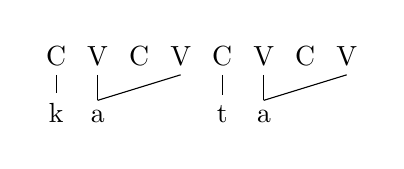
\begin{tikzpicture}
\matrix [matrix of nodes, row sep=0.1em,
column sep={1.5em,between origins}]
{
|(c1)|{C} & |(v1)|{V} & |(c2)|{C} & |(v2)|{V} & |(c3)|{C} & |(v3)|{V} & |(c4)|{C} & |(v4)|{V}      \\[0.6em]
|(C1)|{k} & |(V1)|{a} & |(C2)|{ } & |(V2)|{ } & |(C3)|{t} & |(V3)|{a} & |(C4)|{ } & |(V4)|{ }\\
};
\draw (c1.south) -- (C1.north);
\draw (v1.south) -- (V1.north);
\draw (c3.south) -- (C3.north);
\draw (v2.south) -- (V1.north);
\draw (v3.south) -- (V3.north);
\draw (v4.south) -- (V3.north);
				\end{tikzpicture}
			\xe
		\end{minipage}
		\hfill
		\begin{minipage}{0.5\linewidth}
			\ex \emph{kăta} `fingernail' \\
				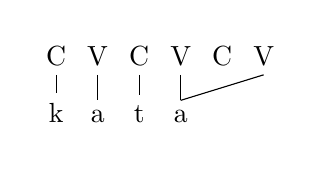
\begin{tikzpicture}
\matrix [matrix of nodes, row sep=0.1em,
column sep={1.5em,between origins}]
{
|(c1)|{C} & |(v1)|{V} & |(c3)|{C} & |(v3)|{V} & |(c4)|{C} & |(v4)|{V}      \\[0.6em]
|(C1)|{k} & |(V1)|{a} & |(C3)|{t} & |(V3)|{a} & |(C4)|{ } & |(V4)|{ }\\
};
\draw (c1.south) -- (C1.north);
\draw (v1.south) -- (V1.north);
\draw (c3.south) -- (C3.north);
\draw (v3.south) -- (V3.north);
\draw (v4.south) -- (V3.north);
				\end{tikzpicture}
			\xe
		\end{minipage}

	What will the stress do? The first /a/ in \emph{kata} `grandma' must get increased prominence. The second V of the long vowel does not project -- length does not matter for stress assignment. When an extra empty CV is inserted, the long vowel cannot associate to it, since it would become super-long. So, the CV is incorporated and then deleted.
	
			\ex \emph{kata} `grandma' \\
				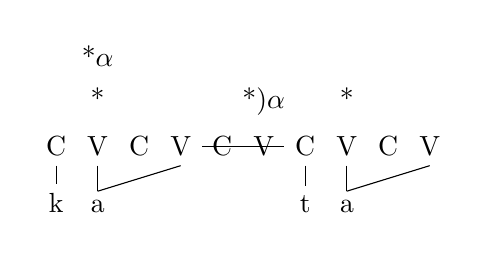
\begin{tikzpicture}
\matrix [matrix of nodes, row sep=0.1em,
column sep={1.5em,between origins}]
{
{} & {*$\alpha$} & {} & {} & {} & {} & {} & {} & {} & {} \\
{} & {*} & {} & {} & {} & {*)$\alpha$} & {} & {*} & {} & {} \\
|(c1)|{C} & |(v1)|{V} & |(c2)|{C} & |(v2)|{V} & |(cs)|{C} & |(vs)|{V} & |(c3)|{C} & |(v3)|{V} & |(c4)|{C} & |(v4)|{V}      \\[0.6em]
|(C1)|{k} & |(V1)|{a} & |(C2)|{ } & |(V2)|{ } & |(CS)|{ } & |(VS)|{ } & |(C3)|{t} & |(V3)|{a} & |(C4)|{ } & |(V4)|{ }\\
};
\draw (c1.south) -- (C1.north);
\draw (v1.south) -- (V1.north);
\draw (c3.south) -- (C3.north);
\draw (v2.south) -- (V1.north);
\draw (v3.south) -- (V3.north);
\draw (v4.south) -- (V3.north);
\draw (cs.west) -- (vs.east);
				\end{tikzpicture}
			\xe	
	When it comes to short vowels, the empty CV can host the geminate: the next consonant will spread onto the empty C-slot.
	
			\ex \emph{kăta} `fingernail' \\
				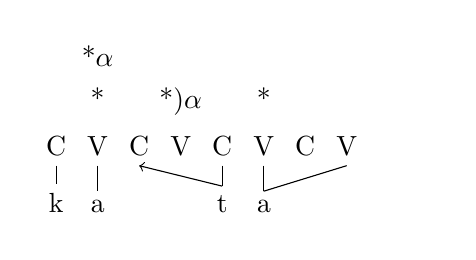
\begin{tikzpicture}
\matrix [matrix of nodes, row sep=0.1em,
column sep={1.5em,between origins}]
{
{} & {*$\alpha$} & {} & {} & {} & {} & {} & {} & {} & {} \\
{} & {*} & {} & {*)$\alpha$} & {} & {*} & {} & {} & {} & {} \\
|(c1)|{C} & |(v1)|{V} & |(cs)|{C} & |(vs)|{V} & |(c3)|{C} & |(v3)|{V} & |(c4)|{C} & |(v4)|{V}      \\[0.6em]
|(C1)|{k} & |(V1)|{a} & |(CS)|{ } & |(VS)|{ } & |(C3)|{t} & |(V3)|{a} & |(C4)|{ } & |(V4)|{ }\\
};
\draw (c1.south) -- (C1.north);
\draw (v1.south) -- (V1.north);
\draw (c3.south) -- (C3.north);
\draw (v3.south) -- (V3.north);
\draw (v4.south) -- (V3.north);
\draw[->] (C3.north) -- (cs.south);
				\end{tikzpicture}
			\xe
			
	In closed stressed syllables with short vowels, there is no gemination, so stress assignment in these contexts should proceed similarly to open syllables with long vowels.
	
			\ex\label{minchisch}\emph{mĭnʹči} `stomach' \\
				\begin{tikzpicture}
\matrix [matrix of nodes, row sep=0.1em,
column sep={1.5em,between origins}]
{
{} & {*$\alpha$} & {} & {} & {} & {} & {} & {} & {} & {} \\
{} & {*} & {} & {} & {} & {*)$\alpha$} & {} & {*} & {} & {} \\
|(c1)|{C} & |(v1)|{V} & |(c2)|{C}  & |(v2)|{V} & |(cs)|{C} & |(vs)|{V} & |(c3)|{C} & |(v3)|{V} & |(c4)|{C} & |(v4)|{V}      \\[0.6em]
|(C1)|{m} & |(V1)|{i} & |(C2)|{nʹ} & |(V2)|{ } & |(CS)|{ } & |(VS)|{ } & |(C3)|{č} & |(V3)|{i} & |(C4)|{ } & |(V4)|{ }\\
};
\draw (c1.south) -- (C1.north);
\draw (v1.south) -- (V1.north);
\draw (c3.south) -- (C3.north);
\draw (c2.south) -- (C2.north);
\draw (v3.south) -- (V3.north);
\draw (v4.south) -- (V3.north);
\draw (cs.west) -- (vs.east);
				\end{tikzpicture}
			\xe		
	Several issues with the analysis featuring the conventional representation of vowel length:
	
	\begin{enumerate}[$\gg$]
		\item If the long vowels are associated to two V-slots even out of stressed environments, why does the length contrast disappear?
		\item Short vowels do not get longer under stress. What will incorporation of the stress CV mean for short vowels?
		\item Why can't the consonant spread in (\ref{minchisch})?
	\end{enumerate}
	
			\subsection{Length only appears in stressed positions}
			
	The alternative is to make both long and short vowels short in the underlying representation. The difference would be in their \emph{potential to associate}: long vowels would spread in the presence of an adjacent empty V slot, whereas short vowels would stay short.
	
		\begin{minipage}{0.4\linewidth}
			\ex \emph{kata} `grandma' \\
				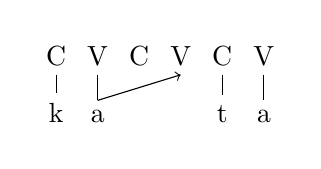
\begin{tikzpicture}
\matrix [matrix of nodes, row sep=0.1em,
column sep={1.5em,between origins}]
{
|(c1)|{C} & |(v1)|{V} & |(c2)|{C} & |(v2)|{V} & |(c3)|{C} & |(v3)|{V}       \\[0.6em]
|(C1)|{k} & |(V1)|{a} & |(C2)|{ } & |(V2)|{ } & |(C3)|{t} & |(V3)|{a} \\
};
\draw (c1.south) -- (C1.north);
\draw (v1.south) -- (V1.north);
\draw (c3.south) -- (C3.north);
\draw[<-] (v2.south) -- (V1.north);
\draw (v3.south) -- (V3.north);
				\end{tikzpicture}
			\xe
		\end{minipage}
		\hfill
		\begin{minipage}{0.5\linewidth}
			\ex \emph{kăta} `fingernail' \\
				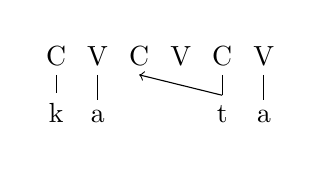
\begin{tikzpicture}
\matrix [matrix of nodes, row sep=0.1em,
column sep={1.5em,between origins}]
{
|(c1)|{C} & |(v1)|{V} & |(c2)|{C} & |(v2)|{V} & |(c3)|{C} & |(v3)|{V}      \\[0.6em]
|(C1)|{k} & |(V1)|{a} & |(C2)|{ } & |(V2)|{ } & |(C3)|{t} & |(V3)|{a}\\
};
\draw (c1.south) -- (C1.north);
\draw (v1.south) -- (V1.north);
\draw (c3.south) -- (C3.north);
\draw (v3.south) -- (V3.north);
\draw[<-] (c2.south) -- (C3.north);
				\end{tikzpicture}
			\xe
		\end{minipage}
		
	\noindent The extra shortness of stress short vowels is caused by gemination of the following consonant; the increased duration of long vowels is an expression of phonological length.
	
	The absence of gemination in closed syllables can be explained if we assume that (a) word-medial empty nuclei (MENs) can be incorporated and (b) the stress CV is not inserted if Line 2 is already filled. The second requirement can be fulfilled if a domain-hood condition is introduced which controls insertion of a stress CV (\ref{dhcond}). 
	
	\ex\label{dhcond}Domain-hood condition for Forest Nenets\\
		A phonological domain must contain a a V-slot that projects to Line 2.
	\xe
	
	If Line 2 is already filled, no CV is necessary; otherwise, it appears in order to be incorporated and to fill Line 2. Similar condition has been proposed by \citeay{ulfsbjorninn2021} for Hawu, where compensatory gemination in stressed syllables is observed, too.
	
			\ex\label{minchisch}\emph{mĭnʹči} `stomach' \\
				\begin{tikzpicture}
\matrix [matrix of nodes, row sep=0.1em,
column sep={1.5em,between origins}]
{
{} & {*$\alpha$} & {} & {} & {} & {} & {} & {} & {} & {} \\
{} & {*} & {} & {*)$\alpha$} & {} & {*} & {} & {} & {} & {} \\
|(c1)|{C} & |(v1)|{V} & |(c2)|{C}  & |(v2)|{V} & |(c3)|{C} & |(v3)|{V}     \\[0.6em]
|(C1)|{m} & |(V1)|{i} & |(C2)|{nʹ} & |(V2)|{ } & |(C3)|{č} & |(V3)|{i}\\
};
\draw (c1.south) -- (C1.north);
\draw (v1.south) -- (V1.north);
\draw (c3.south) -- (C3.north);
\draw (c2.south) -- (C2.north);
\draw (v3.south) -- (V3.north);
				\end{tikzpicture}
			\xe	
			
			\subsection{Representation of the durative}
			
	The durative grows a /mʹ/ after open odd-numbered, and therefore stressed, syllables. Sounds familiar? The proposed representation for the durative contains a floating /mʹ/ that can associate to the stress CV instead of compensatory gemination.
	
		\begin{minipage}{0.4\linewidth}
			\ex \emph{<mʹ>pʹo} `{\Dur}' \\
				\begin{tikzpicture}
\matrix [matrix of nodes, row sep=0.1em,
column sep={1.5em,between origins}]
{
|(v1)|{ }  & |(c2)|{C}  & |(v2)|{V}      \\[0.6em]
|(V1)|{mʹ} & |(C2)|{pʹ} & |(V2)|{o}\\
};
\draw (c2.south) -- (C2.north);
\draw (v2.south) -- (V2.north);
			\end{tikzpicture}
			\xe
		\end{minipage}
		\hfill
		\begin{minipage}{0.5\linewidth}
			\ex \emph{kap°ta-mʹpʹo-sʹ°tu} `invite-{\Dur}-{\Hab}' \\
				\begin{tikzpicture}
\matrix [matrix of nodes, row sep=0.1em,
column sep={1.5em,between origins}]
{
{} & {} & {*$\alpha$} & {} & {} & {} & {} & {} & {} & {} & {} \\
{} & {} & {*} & {} & {*)$\alpha$} & {} & {*} & {} & {} & {} & {} \\
{...} & |(c1)|{C} & |(v1)|{V} & |(c2)|{C}  & |(v2)|{V} & |(c3)|{C}  & |(v3)|{V} & {...}     \\[0.6em]
{...} & |(C1)|{t} & |(V1)|{a} & |(C2)|{mʹ} & |(V2)|{ } & |(C3)|{pʹ} & |(V3)|{o} & {...} \\
};
\draw (c1.south) -- (C1.north);
\draw (v1.south) -- (V1.north);
\draw (c3.south) -- (C3.north);
\draw (v3.south) -- (V3.north);
\draw[<-] (c2.south) -- (C2.north);
				\end{tikzpicture}
			\xe
		\end{minipage}
		
		\section{Schwa as another empty CV}
		
	If schwa is assumed to be a genuine short vowel, its effects are not easy to explain:
	
	\begin{enumerate}[$\gg$]
		\item Gemination happens \emph{after} stressed short vowels but \emph{before} schwa
		\item Schwa is not an incorporating metrical head but rather incorporated itself
	\end{enumerate}
	
	I suggest representing schwa as a CV slot with a floating short /ĭ/. The melodic content is justified by cases where schwa surfaces as a vowel and acts as a harmonic head (\ref{harschwa}).
	
	\ex\label{harschwa} \emph{næpʹaʔk°-hăt°} [næpʹaʰkĭhĭt] ] \hfill `paper-{\Abl}' \xe
	The gemination effect of schwa is produced by spreading the consonant onto the schwa CV. 
	
			\ex \emph{toxoλ°kota} `student' \\
				\begin{tikzpicture}
\matrix [matrix of nodes, row sep=0.1em,
column sep={1.5em,between origins}]
{
{} & {} & {} & {} & {} & {} & {} & {} & {} & {} \\
|(c1)|{C} & |(v1)|{V} & |(cs)|{C} & |(vs)|{V} & |(c3)|{C} & |(v3)|{V} & |(c4)|{C} & |(v4)|{V} & |(c5)|{C} & |(v5)|{V} & {...}     \\[0.6em]
|(C1)|{t} & |(V1)|{o} & |(CS)|{ } & |(VS)|{ } & |(C3)|{h} & |(V3)|{o} & |(C4)|{λ} & |(V4)|{ } & |(C5)|{ } & |(V5)|{ĭ} & {...}\\
};
\draw (c1.south) -- (C1.north);
\draw (v1.south) -- (V1.north);
\draw (c3.south) -- (C3.north);
\draw (v3.south) -- (V3.north);
\draw (c4.south) -- (C4.north);
\draw[<-] (c5.south) -- (C4.north);
\draw[->] (V1.north) -- (vs.south);
				\end{tikzpicture}
			\xe
		
	\begin{enumerate}[$\gg$]
		\item Does the schwa project in this case?
		\item Why is the schwa not pronounced when it makes a geminate?
	\end{enumerate}
	
	The increased prominence effect is caused by incorporation of the schwa. When incorporated, it is not pronounced; this can be ensured by a condition on pronouncing schwa:
	
	\ex Condition on segmental expression of schwa \\
			The short /ĭ/ of the schwa can only be associated to a non-incorporated V-slot.
	\xe
	
			\ex~\emph{naxaλ°} `cone' \\
				\begin{tikzpicture}
\matrix [matrix of nodes, row sep=0.1em,
column sep={1.5em,between origins}]
{
{} & {*$\alpha$} & {} & {} & {} & {*$\beta$} & {} & {} & {} & {} \\
{} & {*} & {} & {*)$\alpha$} & {} & {*} & {} & {} & {} & {*)$\beta$} \\
|(c1)|{C} & |(v1)|{V} & |(c2)|{C} & |(v2)|{V} & |(c3)|{C} & |(v3)|{V} & |(c4)|{C} & |(v4)|{V} & |(c5)|{C} & |(v5)|{V}       \\[0.6em]
|(C1)|{n} & |(V1)|{a} & |(C2)|{ } & |(V2)|{ } & |(C3)|{x} & |(V3)|{a} & |(C4)|{λ} & |(V4)|{ } & |(C5)|{ } & |(V5)|{ĭ} \\
};
\draw (c1.south) -- (C1.north);
\draw (v1.south) -- (V1.north);
\draw (c3.south) -- (C3.north);
\draw (c4.south) -- (C4.north);
\draw[<-] (v2.south) -- (V1.north);
\draw (v3.south) -- (V3.north);
				\end{tikzpicture}
			\xe

\printbibliography
\end{document}